\newpage

\section{绪论}

\subsection{研究背景及意义}
    近几年来,电脑、手机、手环等小型移动设备的大量普及,促进了随着电子技术快速发展,对集成电路的尺寸提出了极高的要求。
    如今,集成电路尺寸最小已经达到14nm,摩尔定律已有失效的迹象。尽管芯片的尺寸在逐年减小,但器单位面积的功率不减反增,
    对产品使用者带来极大困扰。在如此高度集成化的集成电路中,如何降低功耗、提高速度并减小面积逐渐成为了该领域发展的关键与瓶颈。
    \par 模数转换器(ADC)是连接自然界与电子世界的桥梁之一,ADC能够将自然存在的模拟信号,转换为计算机、数字电路可处理分析的数字信号,
    在当今数字化信息化时代充当了不可或缺的角色。无线通讯的过程中,射频信号的收发,都需要经过数据转换电路(ADC与DAC),
    ADC负责将射频电路接收到的电磁波转换为数字波形,供后端数字域设备处理。随着5G时代的到来,对ADC转换器提出了更高的要求。
    一方面,基站密度上升,手机使用量增加,收发毫米波等级的信号,使得芯片的功耗增长巨大。
    另一方面,随着高频频段的引入,超高速、高精度是5G时代ADC不可或缺的特征。
    由于中国集成电路产业起步较晚,该领域仍有较大发展空间,论文中将对一款高速低功耗的ADC进行研究设计。
    \begin{figure}[ht]
        \centering
        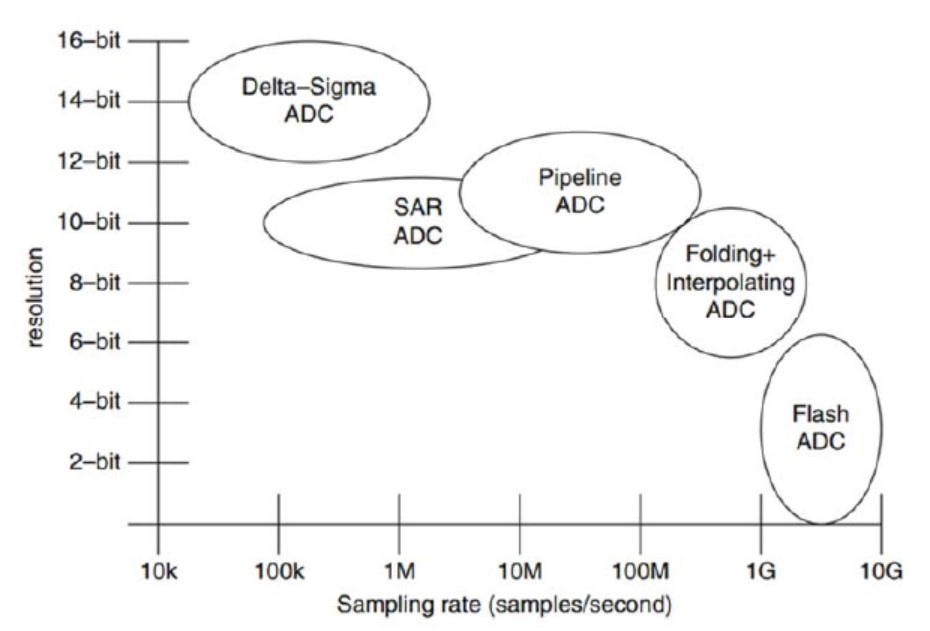
\includegraphics[width=10cm]{AllADC}
        \caption{\label{fig:alladc}不同结构ADC的采样率和分辨率的分布}
    \end{figure}
    \par 如图1.1所示,目前市面上大部分高速ADC均采用Flash ADC,但是其采样精度仅$ 4\sim 6 $bits。
    若要继续提高精度,需要电路中需要大量的比较器,无法满足小面积、低功耗的要求。对于SAR ADC,能够在低功耗
    条件下达到较大的精度,但是速度受限于比较器与DAC的工作速率,对高频段的信号无法处理。
    而Pipeline ADC是一种折中的考虑,其所需比较器数量相对Flash ADC大大减少,同时利用数字校准技术
    能够让分辨率达到较高的标准,同时引入SHA-less架构能够进一步减小芯片功耗以及面积。因此,Pipeline ADC
    往往是高速、高精度ADC的首选。

\subsection{国内外研究现状及趋势}
    Pipeline ADC的研究早在20世纪50年代由Blanchard D. Smith提出,国外至今已有近70年的研究积淀,TI、ADI等公司
    已形成高速、高精度ADC的市场垄断,国内由于起步较晚、发展较慢,暂时没有自主研发的商用芯片,大部分均为学校、研究院
    的研究进展。
    \begin{figure}[ht]
        \centering
        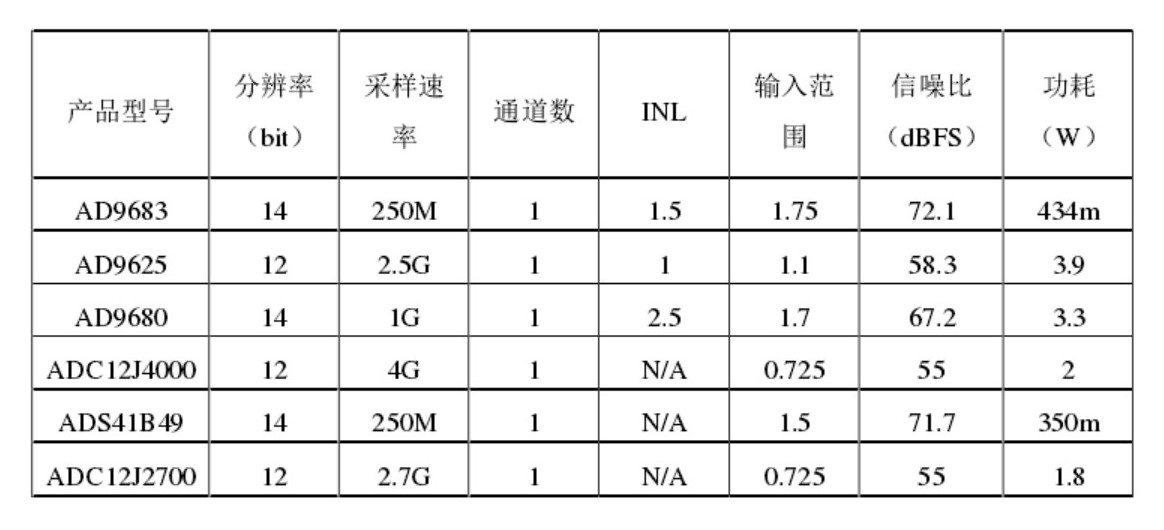
\includegraphics[width=10cm]{ForeignADC}
        \caption{\label{fig:foreignadc}几款国外商用ADC芯片指标}
    \end{figure}
    \par 由图1.2可以看出,国外半导体公司的商用高速高精度ADC能够达到高频的采样速率,大部分都能够达到1GSps。
    \begin{figure}[ht]
        \centering
        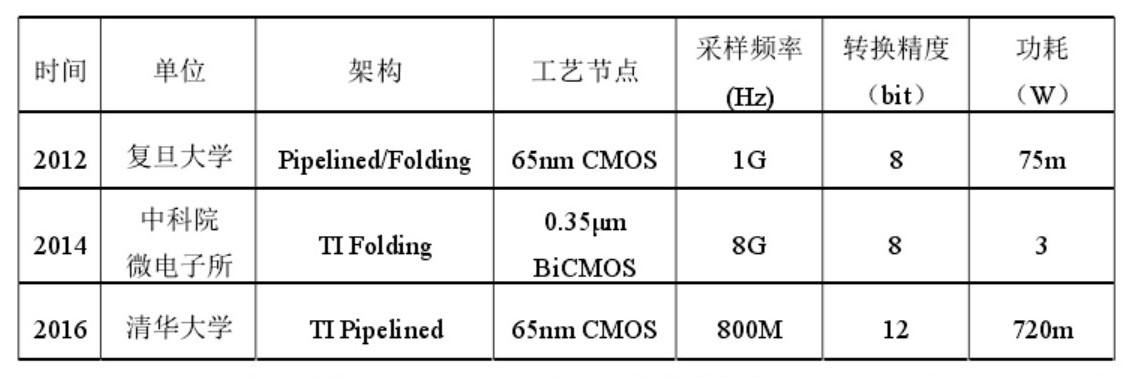
\includegraphics[width=10cm]{HomeADC}
        \caption{\label{fig:homeadc}几款国内研究ADC芯片指标}
    \end{figure}
    \par 由图1.3可知,国内的研究进展仍停留于低速ADC,成果不足。但是以清华大学、复旦大学、
    西安电子科技大学为代表的科研院校,在高速Pipeline ADC方面由一定突破,2016年清华大学
    Xuqiang Zheng等人设计了基于180nm工艺14位250MS/s的中频Pipeline ADC。

